\directlua{pdf.setminorversion(4)}

\documentclass{standalone}
\usepackage{tikz}
\usepackage{tikz-feynman}

\begin{document}

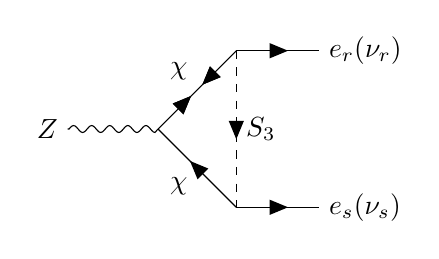
\begin{tikzpicture}
  \begin{feynman}
    \vertex (A) {$Z$};
    \vertex [right=4em of A] (B);
    \vertex [above right=4em of B] (C);
    \vertex [below right=4em of B] (D);
    \vertex [right=3em of C] (E) {$e_{r} (\nu_{r} )$};
    \vertex [right=3em of D] (F) {$e_{s} (\nu_{s} )$};
    \diagram* {
      (A) -- [boson] (B),
      (B) -- [majorana, edge label=$\chi$] (C) -- [charged scalar, edge label=$S_{3}$] (D) -- [fermion, edge label=$\chi$] (B),
      (C) -- [fermion] (E),
      (D) -- [fermion] (F),
    };
  \end{feynman}
\end{tikzpicture}

\end{document}
